% Created 2021-05-10 Mon 18:12
% Intended LaTeX compiler: pdflatex
\documentclass{article}
\usepackage[utf8]{inputenc}
\usepackage[T1]{fontenc}
\usepackage{graphicx}
\usepackage{grffile}
\usepackage{longtable}
\usepackage{wrapfig}
\usepackage{rotating}
\usepackage[normalem]{ulem}
\usepackage{amsmath}
\usepackage{textcomp}
\usepackage{amssymb}
\usepackage{capt-of}
\usepackage{hyperref}
\usepackage[margin=2cm]{geometry}
\usepackage[a4paper,bindingoffset=0.2in,left=1in,right=1in,top=1in,bottom=1in,footskip=.25in]{geometry}
\usepackage[backend=biber,style=apa]{biblatex}\addbibresource{/Users/ricmagno/Documents/References/library.bib}
\addbibresource{/Users/ricmagno/Documents/References/library.bib}
\usepackage{tikz}
\author{Ricardo Antunes, Vicente A. González, Kenneth Walsh, Michael O'Sullivan, and Omar Rojas}
\date{\today}
\title{Productivity Function\\\medskip
\large Mathematical foundation for Production Management in Construction}
\hypersetup{
 pdfauthor={Ricardo Antunes, Vicente A. González, Kenneth Walsh, Michael O'Sullivan, and Omar Rojas},
 pdftitle={Productivity Function},
 pdfkeywords={},
 pdfsubject={Chapter Proposal},
 pdfcreator={Emacs 26.3 (Org mode 9.1.9)}, 
 pdflang={English}}
\begin{document}

\maketitle
\tableofcontents



\section{Guidelines}
\label{sec:org8ad826c}
\begin{verbatim}
(tex-count-word)
\end{verbatim}
\begin{itemize}
\item 7000 Words
\end{itemize}

\section{Abstract}
\label{sec:org54c07ad}
The building construction industry faces challenges, such as increasing project complexity, and larger scope requirements but shorter deadlines. 
Additionally, the industry relies on practices based on intuition and experience, overlooking the dynamics of its production system. 
These approaches underestimate the influence of process repetitiveness, the size of the production run, the transient state (setup times), the variation of learning curves, and the conservation of processes properties. 
Consequently, construction adopts the manufacturing production model dismissing the application of approaches that accurately describe the characteristics of its production system. 
This chapter aims to provide a production theory to better understand the production mechanisms of repetitive processes in project-driven systems in construction.
The chapter begins with an examination of the existing knowledge about production models, their characteristics, and the challenges to establishing a theoretical framework for controlling dynamic production systems management in construction projects. 
The chapter progresses to an analytical and scalable method (Productivity Function) to represent the behavior of production systems. 
The Productivity Function provides a mathematical foundation for the calculations of cycle times (average, best- and worst-cases), throughput at capacity, and the influence of the transient state time in the production variability. 
Productivity Function is applied in feedback loop control yielding a robust approach to plan, control, and optimize production.
Finally, the chapter presents automated methods of data collection that feed the Productivity Function models, which are the foundation of the production theory and support the decision-making process on Lean Construction 4.0. 

\section{Introduction}
\label{sec:org224f97c}
Despite the name of the title of this chapter, you will not find equations here.
Not because they do not exist, but because we believe that, at least for now, it is more important to understand what these equations represent than how they come to be.
You are welcome to deep your knownledge and see the equations and their development on the referenced literature.
\section{Lean principles and production theory [0/2]}
\label{sec:org2996b78}
\subsection{Production in manufacturing (Factory Physics)}
\label{sec:orga1dc28b}
The manufacturing industry is knowable of its production.
From early times when 'time and motion' has been developed on workers construction a brick wall (Reference here), manufacturing has being advancing on undestanding and manageming of its production.
Mostly important on the context on this book, it was the creation and development of lean production that inspired lean construction.
This chapter stands on further development of lean production: it's mathematical explanation of production.
Such work has been conducted by TOYOTA dude, THE guy from MIT and mates from Factory Physics.
Their work combined provide a set of equations that apply to manufacturing production systems.
A production system consists into three main elements: inputs, process, outputs (Figure ).
Inputs may not reflecet the full range of requirementes to create the output but on this system view they determine the output.
The process can be determined on physical knwon equations or most oftern determined by evaluating the relationship betwen input and output.
The mathematical representation of this relantionship is main difference between manufacturing and construction.

\subsection{The manufacturing theory does not apply directly to construction}
\label{sec:orgf82a055}

Manufacturing is either a continous or a repective process.
Machinery and human resources are specialized and qualified.
Production flow and material routes are established. 
Thus, most manufacturing processess can be automated.
That scenario is different from construction.
While capacity is knwon and measured in manufacturing, there was no way to measured it in construction.
Increasing production in construction often means add more human resources.
That often cause decrease of productivity due to lack of space, tools, skills, etc.
\section{Productivity Function [0/4]}
\label{sec:org13931d9}
\subsection{Production process system representation [100\%]}
\label{sec:orgaec9f55}

\uline{Source Paper07}

Several elements found in this literature review connect the characteristics of construction projects to the characteristics of a dynamic system.
As shown in Figure 4, the interconnectivity is explicit between project stages, in the event that subsequent phases rely on the accomplishment and performance of previous ones.
This dependent connection remains valid for divided n-substages or n-activities and also applies to the proposed framework.
The dependence of processes and/or activities is well documented in the literature and well known by practitioners.
An activity or stage may impair or favour a successive action depending on the level of correlation and dependence.
The interdependence of activities forms a conduit to the propagation of unsure events. Potential risks captured through the entire project life may impact project execution whenever not properly treated, resulting in project deviations.
This sequence of events is represented in the system by the flow of uncertainty to risk and the occurrence of risk events, through risk management filtering actions—avoidance, acceptance, sharing, transference, mitigation, motivation—and, finally, to variability.
This flow resembles an intrinsic characteristic of systems in the presence of disturbance or noise.
Control systems may transmit unfiltered noise across connections affecting vulnerable components and causing disturbances or unpredicted behaviour.
Although the level of influence in this flow of sequential, parallel or overlapping relationships in the process or activity network have not been investigated at this point, understanding how risk transforms into variability, and especially how variability affects networked activities, propitiates an opportunity to develop methods aimed at avoiding and mitigating (filtering) the propagation of risk (noise). Regarding risk materialization in variability, different outcomes build on how concentrated or distributed the risk impact was.
This scenario requires a function capable of scale variation and energy conservation (impact) when calculating the functional energy.
The wavelet network evolved from the Fourier transformation: “wavelet network is a type of building block for approximation of unknown functions based on the concept of the multi-resolution approximation.
The building block is formed by shifting and dilating the basis functions, the mother wavelet and father wavelet” [97].
A wavelet network may be used as universal function approximator (“a universal function approximator is a system that, given a set of predictor variables, can output an accurate estimate of some predicted variable” [97]) to estimate unknown nonlinear functions and to attain a required control performance.
A new concept in the control area, wavelets have been successfully used in several applications, such as physics, signal processing and statistics, where small complicated details matter [98].
Operating on possibly the same conditions of wave theory—linear/nonlinear, deterministic/stochastic, time-domain/frequency domain, direct/inverse problems, discrete/continuous models [99]—control theory may create a proxy theory to explain the effects of variability in construction projects by extending the elements of the dynamic systems.

\#+BEGIN\textsubscript{LATEX}:
\begin{figure}
  \centering
  \begin{tikzpicture}[>=latex',every node/.append style=
      {font=\scriptsize},node distance=5mm]

  \node [input, name=input] {};
  \node [sum, right=12mm of input] (control_sum) {};
  % \node [block, right=12mm of control_sum, rounded corners] (K) {Controller \\ $K$};
  \node [block, right=3cm of control_sum, rounded corners] (G) {System \\ $G$};
  \node [dot, right=12mm of G] (snodo1) {};
  \node [output, right=of snodo1] (output) {};

  \begin{scope}[auto]
    \draw [->] (input) -- (control_sum)
    node[very near start] {$r(t)$}
    node[very near start,swap] {Reference}
    node[very near end] {$+$};
    % \draw [->] (control_sum) -- node {$e(t)$} node[swap] {Error} (K);
    \draw [->] (control_sum) -- node {$u(t)$} node[swap] {Input} (G);
    \draw [-] (G) -- node {$y(t)$} node[swap] {Output} (snodo1);
    \draw [->] (snodo1) -- (output);
    \draw [->] (snodo1) |- +(0,-1.5) -| (control_sum)
    node[near start]{}
    node[near start, swap]{}
    node[very near end] {$-$};
  \end{scope}
  \end{tikzpicture}
  \caption{Feedback loop}\label{fig:Feedback loop}
\end{figure}
\#+END\textsubscript{LATEX}





\url{./Figures/Construction\_project\_driven\_production\_system.weps}

\begin{figure}[htbp]
\centering
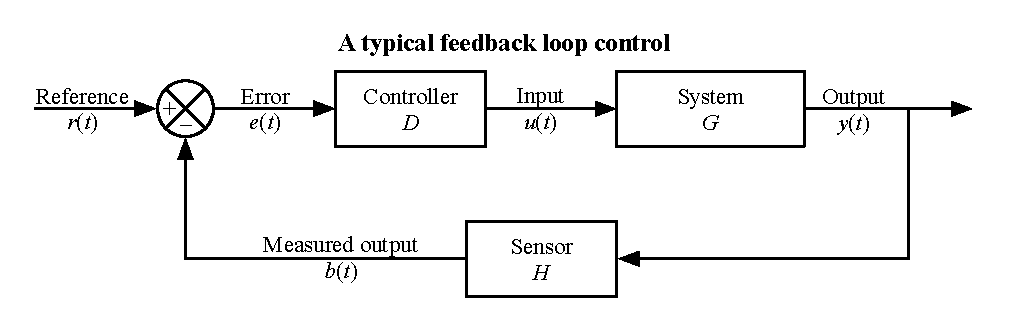
\includegraphics[height=150]{./Figures/A_typical_feedback_loop_control.eps}
\caption{\label{fig:org443301d}A typical feedback loop control}
\end{figure}


The simplest model of construction processes considers a closed conversion process where all factors affecting the work are steady state \cite{Drewin1982}.
In this model, the relationship between output and input, i.e., productivity, is given by a constant which is unaffected by external factors.
This constant can be determined by, for instance, the linear curve fitting or the ratio of the sum of outputs to the sum of inputs.
The linear scheduling method (LSM) \cite{Harmelink1998,Su2016} and line-of-balance (LOB) \cite{Lumsden1968,Su2016,ZolfagharDolabi2014} are examples of scheduling models for repetitive processes based on the steady state model.
However, ``because of the steady state nature of this model, the system more closely represents industrial production processes than construction processes \cite{Thomas1990}.'' Short production runs \cite{Bashford2005}, high levels of output and input variability \cite{Gonzalez2009}, and nonlinear input-output relationships \cite{Bertelsen2003,Lutz1993} frequently prevent repetitive production processes in construction to reach steady state \cite{Antunes2015a,Walsh2007}.

\subsection{Mathematical foundation of the Productivity Function}
\label{sec:org3316295}

Although much work has been done on production management of repetitive construction processes, more studies need to be conducted to develop equations to quantify project-driven production systems in construction.
The objective of this paper is to formulate variants of manufacturing production equations to calculate the production performance of repetitive construction processes for benchmarking purposes.
Furthermore, this paper shows the calculation of theoretical production parameters such as capacity and cycle time, as well as the influence of transient time on productivity.
The contribution of this paper to the body of knowledge are algebraic equations based on a generic model to calculate production parameters for repetitive processes in construction.
\subsubsection{TODO Explain transient and steady-state}
\label{sec:orgd8a4ae4}

\begin{enumerate}
\item Mathematical foundation of production
\label{sec:orgbea4530}

Repetitive construction projects falls into a fuzzy area where both project management and manufacturing overlap.
Repetitive construction projects are constituted by several contractors executing processes that they are specialized in, as for instance plumbers and electricians, that in the end, build a one-of-a-kind product.
The operations executed by several contractors are often performed repeatedly, and simultaneously at times, which stands for one of the peculiarities of repetitive projects.
In project-driven production, the coexistent mix of characteristics from project management and manufacturing makes the management of project-driven production problematic.
Project-driven production systems, such as repetitive construction, involve a combination of processes at transient, unsteady state, and-rarely-at steady state \citep{Antunes2015a,Antunes2015,Bashford2005,Walsh2007}.
However, traditional construction management, at this time, utilizes practices based on the manufacturing model that lacks the mathematical foundation to model and manage production in the project-driven systems \citep{Bertelsen2003,McCray2002,Pereira2013,Ko2016}.

\begin{itemize}
\item The system steady-state.
The steady-state of a system
\end{itemize}

\item Explain traditional methods of steady-state
\label{sec:org6370d98}
The transient is the immediate system reaction of an input change from a rest state \citep{Ogata2010}.
If the system is stable, the response will tend to a constant value, \(y_{\mbox{ssv}}\), when the time, \(t\), goes to infinity (Equation\textasciitilde{}\ref{eq:steady state}).
When the output reaches this value, the response is then at steady state.
The time that the system response takes from the moment the input changes to the steady state \citep{Nise2010,Ogata2010}, is the settling time, \(t_s\), i.e., the duration of the transient state.
Figure\textasciitilde{}\ref{fig:Transient} shows the step analysis which is an artificial and controlled way to reproduce the transient, as well as determine the steady state response of a system represented by the Productivity Function.
In the unitary-step function, \(u_{\mbox{step}}(t) \overset{\underset{\mathrm{\mathcal{L}}}{}}{\leftrightarrow} U_{\mbox{step}}(s) = 1/s\), at a time \(t_0\) the input changes from 0 to 1 and then is kept constant at 1.
At \(t_0\), if there is no delay, the system will notice the change in the input generating the transient response.
A physical interpretation of the step function is switching on a light by pressing a button.
Finally, if the system is stable; the output will tend to the steady state value.

\begin{equation}\label{eq:steady state}
	y_{\mbox{ssv}} = \lim_{t\rightarrow \infty} y(t)
\end{equation}


\begin{figure}[htbp]
\centering
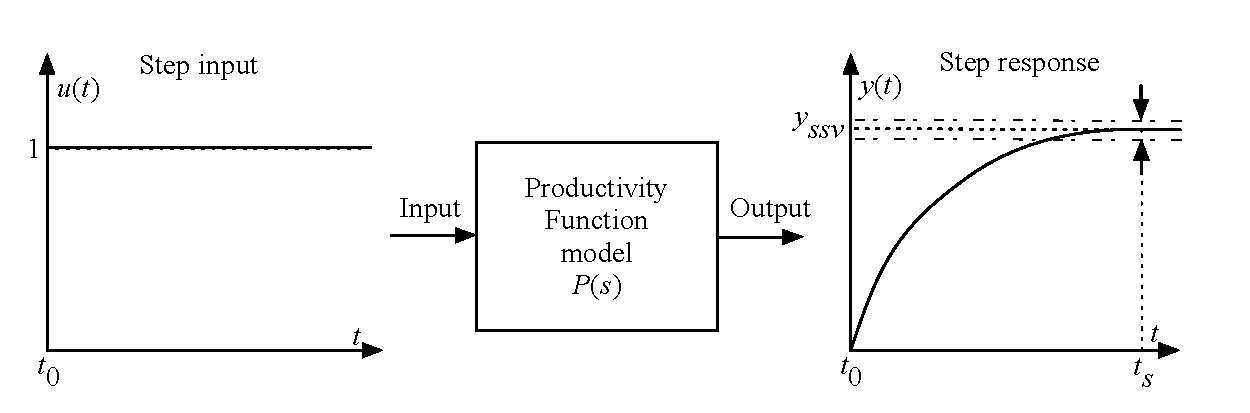
\includegraphics[height=150]{./Figures/FIG02Transient_analysis.eps}
\caption{\label{fig:org4dfd80d}Transient analysis for unit step input \label{fig:Transient}}
\end{figure}


The step function in the time domain is given by:

\begin{equation}\label{eq:Step function in time domain P7}
	u_{\mbox{step}}(t) =
	\begin{cases}
 	0, & t = 0 \\
  1, & t \ne 0
	\end{cases}.
\end{equation}

The production of products or services designed to fulfill unique, or one-of-a-kind, specifications is the essence of project-driven production, also known as project-oriented manufacturing \citep{Martinez1997}.
``Repetitive construction projects are resource-driven, multi-unit projects characterized by activities which need to be performed in a sequence from unit to unit repeatedly \citep{Hajdasz2015}.'' That assumes a position in Product process matrix (Figure\textasciitilde{}\ref{fig:F01}) between manufacturing and project management, hence mixing characteristics from both sides, following the manufacturing production structure on the make-to-order (or make-to-build) demand of projects.
The product-process matrix (Figure\textasciitilde{}\ref{fig:F01}) illustrates the relationship of different products regarding their workflow and volume.
The most visible characteristic of the figure is a diagonal arrangement of the products showing a directly proportional relationship between production volume and workflow connection \citep{Kumar2009}, and also a relationship between the degree of freedom and production focus.

At the lower end of the diagonal, products are produced in high volume units and with hardly any or no differentiation at all, e.g., commodities.
Furthermore, the production process matches the characteristics of long run production \citep[p.154]{Baye2010} and economies of scale \citep[p.185]{Baye2010}.
The work stream is a continuous flow of specialized processes and equipment running at peak efficiency with stable and low variation processes \citep[pp.8-10]{Hopp2001} and relative short transients.


\begin{equation}\label{eq:Productivity_Function}
	P(s) = \frac{Y(s)}{U(s)} =
	\frac{(\beta_m s^m + \beta_{m-1} s^{m-1}+\ldots+\beta_0)}{(\alpha_n s^n + \alpha_{n-1} s^{n-1}+\ldots+\alpha_0)}
\end{equation}
\end{enumerate}

\subsection{Modelling method [0/0]}
\label{sec:org648f953}
\uline{Source Paper04}

The objective of system identification is to build mathematical models of dynamic systems using measured data from a system \citep{Ljung1999}.
There are several system identification approaches to model a variety of systems; for instance, transfer function.
The transfer function is particularly useful because it provides an algebraic description of a system as well means to calculate parameters of the system dynamics and stability.
Nevertheless, the modeling capability of the transfer function in construction must be evaluated and tested.
In this study, the modeling approach, i.e., transfer function, focuses on replicating the input/output `mapping' observed in sample data.
When the primary goal is the most accurate replication of data, regardless of the mathematical model structure, a black-box modeling approach is useful.
Additionally, black-box modeling supports a variety of models \citep{Bapat2011, Billings2013}, which have traditionally been useful for representing dynamic systems.
At the end of the black-box modeling, a mathematical description represents the actual process performance rather than a structure biased by assumptions and restrictions.
Black-box modeling is a trial-and-error method, where parameters of various models are estimated, and the output from those models is compared to the results with the opportunity for further refinement.
The resulting models vary in complexity depending on the flexibility needed to account for both the dynamics and any disturbance in the data.
The transfer function is used to show the system dynamics explicitly.

\subsubsection{Step response: Transient and steady state}
\label{sec:orgbd66aa2}

The transient is the immediate system reaction of an input change from a rest state \citep{Ogata2010}.
If the system is stable, the response will tend to a constant value, \(y_{\mbox{ssv}}\), when the time, \(t\), goes to infinity (Equation\textasciitilde{}\ref{eq:steady state}).
When the output reaches this value, the response is then at steady state.
The time that the system response takes from the moment the input changes to the steady state \citep{Nise2010,Ogata2010}, is the settling time, \(t_s\), i.e., the duration of the transient state.
Figure\textasciitilde{}\ref{fig_FIG02StepAnalysis} shows the step analysis which is an artificial and controlled way to reproduce the transient, as well as determine the steady state response of a system represented by the Productivity Function.
In the unitary-step function, \(u_{\mbox{step}}(t) \overset{\underset{\mathrm{\mathcal{L}}}{}}{\leftrightarrow} U_{\mbox{step}}(s) = 1/s\), at a time \(t_0\) the input changes from 0 to 1 and then is kept constant at 1.
At \(t_0\), if there is no delay, the system will notice the change in the input generating the transient response.
A physical interpretation of the step function is switching on a light by pressing a button.
Finally, if the system is stable; the output will tend to the steady state value.

\begin{equation}\label{eq:steady state}
	y_{\mbox{ssv}} = \lim_{t\rightarrow \infty} y(t)
\end{equation}

The step function in the time domain is given by:

\begin{equation}\label{eq:Step function in time domain P7}
	u_{\mbox{step}}(t) =
	\begin{cases}
 	0, & t = 0 \\
  	1, & t \ne 0
	\end{cases}.
\end{equation}

\subsection{Production Theory for Construction}
\label{sec:orgf1d3594}
\subsubsection{Production forecast}
\label{sec:org67e6666}

Forecasting is a tool that allows managers to create and access different scenarios of production result of risk impact.
Hence, forecasting supports both risk management practices for mitigating risk as the result of current progress on future completion.
Even though forecasting in construction is often inadequate and one of the weakest project controls functions \citep{ConstructionIndustryInstitute2012}.
``While there are many reasons for poor forecasting practice, one of the main causes may be the limited educational resources available on forecasting
In many textbooks and manuals, education about forecasting starts and stops with a presentation of earned value and elementary trending calculations \citep{ConstructionIndustryInstitute2012a},'' such as linear functions and averages.
The numerical estimation approach of Productivity Function can be embedded in the Project Management software or used as a stand-alone tool to forecast, access and simulate critical processes that require in-depth project controls.
As the Productivity Function models do not require anything else than the process' inputs and outputs, e.g., labor hours used to produce square meters of plastered wall, the models can be used together with project control practices such as earned value or Planned Percent Complete (PPC).
Simply by replacing the traditional steady state model by the Productivity Function, more accurate results should be obtained.
Furthermore, Dynamics Simulation, which relies on the mathematical models defined by ordinary differential equations (as the Productivity Function), have a significant role in supply chain \citep{Higuchi2004} and production in manufacturing \citep{Forrester1997}.
The application of Dynamics Simulation in construction is rare, specifically due to the lacking of mathematical models to describe the production in construction.
A gap that may be fulfilled by the Productivity Function.
While the algebraic form of Productivity Function may support the development of equations that further explain the production of project-driven processes, such as equations for capacity and cycle time.
Furthermore, the measurement and visualization of the transient state of project-driven processes support the quantitative and structured application of methods to reduce setup times, as for instance, Single Minute Exchange of Dices (SMED) and pre-fabrication \citep{Antunes2016}.

This chapter initiated as an exploration of elements in the building construction project cycle and their effect on production behavior, resulting in theoretical framework structured as a system \citep{Antunes2015a}.
This system proposed a flow of uncertainty to risk and then risk impact risk impact that would cause variability.
Following the framework, an analytical technique to describe the dynamic conditions of production in repetitive processes in projects was suggested \citep{Antunes2015}, as well as the relationship between the model characteristics and flow variability \citep{Antunes2016}.
This study is a step forward towards the development of a mathematically driven production theory for construction project management and project-driven systems defining a modeling approach and pointing out that dynamical systems theory would be useful to describe the behavior of production in construction.

\subsubsection{Variability analysis}
\label{sec:orgdbd5ca1}
``Law (Variability): Increasing variability always degrades the performance of a production system \citep{Hopp2001}.''
In other words, the system will achieve its maximum performance when there is no variability.
That becomes evident when analyzing CV (Equation\textasciitilde{}\ref{eq:CV}): the greater the coefficient of variation, CV$\backslash$@; lower is the mean output, \(\bar{y}\), i.e., \(\bar{y} \sim \mbox{CV}^{-1}\).
Based on the knowledge of dynamic systems, the lowest level of variation in the output (indistinctly used in this paper as throughput once the outputs of dynamic systems are time dependent) happens when the system is at steady state \citep{Nise2010,Ogata2010}.
Productivity Function can be used to determine the theoretical output at steady state, and consequently the cycle time, using the stationary conditions as shown in Equation\textasciitilde{}\ref{eq:LongRun}.

The output at steady state of a system represented by a Productivity Function in the frequency domain can be calculated using the final value theorem.
``The final value theorem provides an easy-to-use technique for determining this value without having to first invert the Laplace transform to determine the time signal \citep[p.97]{Chen2007}.''
Equation\textasciitilde{}\ref{eq:FinalValue} shows the final value theorem which gives the steady state value, \(y_{\mbox{ssv}}\), in the frequency domain.

\begin{equation}\label{eq:FinalValue}
	\lim_{t\rightarrow \infty} y(t)=\lim_{s\rightarrow 0} sY(s)
\end{equation}

Replacing \(Y(s) = U_{\mbox{step}}(s) \times P(s)\), where \(U_{\mbox{step}}(s)\) is the step function, \(1/s\): \(Y(s) = 1/s \times P(s)\)

\begin{equation}\label{eq:FinalValue2}
	\lim_{t\rightarrow \infty} y(t)=\lim_{s \rightarrow 0} s \frac{1}{s} \times P(s)
\end{equation}

Replacing the left side of the Equation\textasciitilde{}\ref{eq:FinalValue2} by Equation\textasciitilde{}\ref{eq:steady state} the result is the output at steady state, i.e., the system's highest throughput with lowest variation: capacity.

\begin{equation}\label{eq:Capacity}
	y_{\mbox{ssv}} = \lim_{s \rightarrow 0} P(s) = P(0)
\end{equation}

\subsubsection{Production benchmark}
\label{sec:org290f339}
\subsubsection{Production plan, monitoring, and control}
\label{sec:org48f792d}
\begin{enumerate}
\item Throughput
\label{sec:org1e8c937}
Throughput is the output (non-defective) of a production process in a defined period \cite{Hopp2001}.
Construction scheduling accuracy strongly depends on being able to coordinate resources to determine the processes throughput \cite{Cho2011}.
When the relationship between resources and throughput can be established;
it is possible to determine the necessary resources to achieve the desired performance \cite{Cho2011}.
The production workflow in construction is segmented, i.e., job shop, where ``jobs arrive in different forms and require different tasks, and thus the equipment tends to be relatively general purpose \cite{Hayes1979},'' equipment has different productivity/availability \cite{Ok2006}, and the increased labor resource frequently causes site congestion \cite{Cho2011}.
There is an endless list of human factors that influence the labor output, such as the workers' experience, skill, and age \cite{El-Gohary2014}.

The open conversion model \cite{Kellogg1981} considers internal, external, and also unknown influences to productivity in a hierarchical arrangement.
Despite being generic and industry-comprehensive, at the operational level the complexity of inputs, such as the cost of labor, capital, energy, and materials; and output, e.g., dollars, makes the use of the open conversion model impractical \cite{Thomas1990}.
Explicitly incorporating all factors that influence productivity in a model is a challenging task.

``The relationship between inputs and outputs is very complex and, in many cases, includes some unknown combined effects \cite{Ok2006}.''
Simplifications and assumptions have to be made; however, the models are often over simplified.

\item Cycle-time
\label{sec:org7f568c7}





The accumulated throughput over time results in units of a service or product produced over time.
The time taken to produce one output is the cycle time.
In a continuous system, the function of the output produced is given by the integral of the output.
At steady state, where the throughput is constant, the unitary area below the curve is given by the throughput, \(y_{\mbox{ssv}}\), multiplied by the cycle time (Equation\textasciitilde{}\ref{eq:Capacity}).
In other words, the area results from the time when the last output was produced, \(t_{j-1}\), minus the time when the production of the current output unit finishes \(t_j\), where \(j\) is the denotation of an element and \(j \in N^+\).
Hence, \(\Delta t_j=t_j-t_{j-1}\) is the time taken to produce the \$j\$th-output, i.e., cycle time, \(\mbox{CT}_j\).
Therefore, Equation\textasciitilde{}\ref{eq:CycleTime} is equivalent to Equation\textasciitilde{}\ref{eq:CT}.
As \(y_{\mbox{ssv}}\) should determine the capacity of the system, the cycle time at steady state is the shortest production time of the system while stable, i.e., cycle time (best).

\begin{equation}\label{eq:CycleTime}
	y_{\mbox{ssv}} \times (t_j-t_{j-1}) = 1, \quad\mbox{ or }\quad \Delta t_j = 1/y_{\mbox{ssv}}
\end{equation}

Different to the steady state, the throughput of the production system varies while the system is in the transient.
The unitary area under the throughput curve can be calculated by a limited integral, with \(t_{j-1}\) and \(t_j\) as lower and higher limits, respectively (Equation\textasciitilde{}\ref{eq:ArtifactJ}).
As the throughput decreases, the cycle time increases.
Hence, the maximum cycle time of the production system, i.e., cycle time (worst) is found at start-up when the throughput at time \(t_0\) is null.

\begin{equation}\label{eq:ArtifactJ}
	\psi_j = \int_{t_{j-1}}^{t_j} y(t)dt
\end{equation}

Considering that the production system will increase its throughput over time as per its transient curve; the cycle time (worst) is the time taken to produce the first output (\(j=1\)) from a rest state: \(\Delta t_m = t_1-t_0\), or simply \(\Delta t_j = t_1\), once \(t_0 = 0\), is given by Equation\textasciitilde{}\ref{eq:Artifact1}.

\begin{equation}\label{eq:Artifact1}
	\psi_1 = \int_{0}^{t_1} y(t)dt
\end{equation}

Consequently, if the process increases its throughput as described by its transient curve, the longer it will take to reach the steady state and the smaller will be the area under the curve; hence, smaller its average output produced per time.
The average output per time can be calculated by the average function value given by Equation\textasciitilde{}\ref{eq:Artifact2}.

\begin{equation}\label{eq:Artifact2}
	\psi_{t_s} = \frac{1}{t_s} \int_{0}^{t_s} y(t)dt
\end{equation}

In other words, for processes with equal capacity, \(y_{\mbox{ssv}}\), the longer the transient time, \(t_{s}\), the longer is the average cycle time, \(\bar{\mbox{CT}}\).
Also, for processes with equal transient time the greater the capacity, the smaller is the average cycle.

\begin{equation}\label{eq:CycleTime}
y_{\mbox{ssv}} \times (t_j-t_{j-1}) = 1, \quad\mbox{ or }\quad \Delta t_j = 1/y_{\mbox{ssv}}
\end{equation}

\begin{enumerate}
\item Average cycle-time
\label{sec:org566424e}
\item Worst cycle-time
\label{sec:org411cc13}
\item Best cycle-time
\label{sec:orgaa73bab}
\end{enumerate}
\item Capacity
\label{sec:org79a68d1}
``Law (Capacity): In steady state, all plants will release work at an average rate that is strictly less than the average capacity \citep[p.]{Hopp2001}.''
Furthermore, in most cases, releasing work into the system above the capacity causes the system to become unstable \citep{Hopp2001}.
According to these definitions, it would be correct to state that a process' capability is the highest throughput achievable without the process becoming unstable.
Thus, at capacity, the process operates with optimal productivity \citep{Kisi2017}.
``The theoretical maximum productivity that would be achieved under absolutely perfect conditions in all respects (perfect weather, highly motivated, and productive labor with perfect workmanship, optimal materials, optimal equipment, no interferences from other trades, no design errors, perfect understanding of design intend, etc \ldots) \citep[p.150]{Son2011}.''

However, the variation in the efficiency of workers and equipment, actual demand, and scheduling planning and control\textasciitilde{}\cite[p.54]{Kumar2009} may prevent processes from achieving the system design capacity.
Design capacity in a manufacturing system is engineered to full-scale operating conditions.
However, the system capacity is less than the design capacity, because the full-scale operating conditions are rarely met \citep{Kumar2009}.

The capacity of project-driven processes is not engineered but based on intuition \citep{McCray2002,ProjectManagementInstitute2011}.
Regardless of the equation used for productivity measurement \citep{Thomas1990}, determining the system capacity is crucial to settling a benchmark and elaborating what the level of productivity the actual performance should be compared to \citep{Abdel-Razek2007,Olomolaiye1998,Zhao2014}.



\begin{equation}\label{eq:Capacity}
	y_{\mbox{ssv}} = \lim_{s \rightarrow 0} P(s) = P(0)
\end{equation}
\end{enumerate}


\section{Applicability}
\label{sec:org9563ed3}
\subsection{Automation and technology}
\label{sec:org0e5c59d}
\subsubsection{Supervisory control and data acquisition (SCADA)}
\label{sec:org6e7b27c}
\subsubsection{Challenges}
\label{sec:orge225211}
\subsection{Decision-making support}
\label{sec:orgd531890}
\subsection{Benefits and impacts}
\label{sec:orgac622fe}
\section{Discussion}
\label{sec:org40d2b1f}
\section{Conclusion}
\label{sec:org38f47e8}

\section{References}
\label{sec:org00fcb0a}

\printbibliography[title=none]
\end{document}